\documentclass[12pt,a4paper]{article}
\usepackage[utf8]{inputenc}
\usepackage{amsmath}
\usepackage{amsfonts}
\usepackage{amssymb}
\usepackage{graphicx}
\usepackage{booktabs}
\usepackage{natbib}
\usepackage{dcolumn}
\usepackage{setspace}
\usepackage{array}
\usepackage{pdflscape} %allows for rotating pages with wide tables
\newcolumntype{P}[1]{>{\raggedright\arraybackslash}p{#1}}
\usepackage{tabulary}
\usepackage[T1]{fontenc}
\usepackage{lmodern}
\usepackage[protrusion=true,expansion=true]{microtype}
\usepackage[top=1.5in, bottom=1.5in, left=1in, right=1in]{geometry}
\usepackage{todonotes}

%%% these three may have to be commented back in when submitting
%\usepackage{endnotes}
%\let\footnote=\endnote
%\usepackage[heads,nolists,tablesfirst]{endfloat} %places tables and figures at the end

\usepackage{mathptmx}
\usepackage{soul}
\usepackage{color}
\usepackage{hyperref}
\usepackage[font={footnotesize}]{caption}
%\usepackage{adjustbox} %for centering tables


\title{ \textbf{Intergroup Bias \\ in Parliamentary Rule Enforcement}  }

\author{Frederik Hjorth\thanks{Corresponding author. Department of Political Science, University of Copenhagen, Øster Farimagsgade 5, DK-1353 Copenhagen K, (+45) 26 27 24 41, \texttt{\href{mailto:fh@ifs.ku.dk}{fh@ifs.ku.dk}}}}

\date{}

%\corref{cor1}} \ead{fh@ifs.ku.dk}

\begin{document}

\maketitle


%\begin{center}
%	\textsc{draft -- please do not quote, cite, or distribute}
%\end{center}

%\cortext[cor1]{ Øster Farimagsgade 5, DK-1353 Copenhagen K, (+45) 26 27 24 41}
%\tnotetext[t1]{The author would like to thank Michael Lewis-Beck, Peter Dinesen, Martin Vin\ae s, Yosef Bhatti, and Mads Dagnis Jensen for helpful comments on earlier drafts of this paper. The usual disclaimer applies.} 
%\address[cph]{University of Copenhagen}

\doublespacing

\begin{abstract}
\noindent Political actors are often required them to enforce rules without giving in-groups special treatment. But are such institutional roles likely to be successful? Here, we exploit a special case of exogenously assigned intergroup relations: debates in the Danish parliament, in which parliament chairmen drawn from parliamentary parties enforce speaking time. Analyzing 5,756 speeches scraped from online transcripts, we provide evidence that speech lengths are biased in favor of the presiding chairman's party. On average, speakers of the same party as the presiding chairman give 5 percent longer speeches and are 5 percent more likely to exceed the speaking time limit. The paper contributes to the extant literature by demonstrating political intergroup bias in a natural setting, suggesting that group loyalties can supersede institutional obligations even in a `least likely' context of clear rules, complete observability, and a tradition of parliamentary cooperation.
\end{abstract}

%\begin{keyword}
%\doublespacing
%legislatures \sep debates \sep intergroup bias \sep rule enforcement \sep social identity
%\end{keyword}
%
%\end{frontmatter}


%\onehalfspacing

\newpage

\section{Introduction}

\noindent In a variety of contexts, institutions accord individuals formal roles which require them to enforce rules governing the competing interest of societal groups. In some cases, by either design or necessity, these individuals are drawn from one of the groups subject to these rules. Hence, in order to enforce the rules in an unbiased manner, assuming the role requires the individual to disregard his or her group loyalties. 

But are such institutional roles and norms likely to be successful? In this study, we exploit a natural experiment in rule enforcement where the enforcer belongs to a group subject to enforcement. The empirical setting is parliamentary debates in Denmark, in which speaking times, governed by a simple, uniform rule, are enforced by chairmen drawn from major political parties.\footnote{In the interest of fluency, the paper refers to both chairmen and -women using male pronouns, reflecting the modal speaker gender.} Since combinations of speakers and chairmen are effectively random, the setting allows for identifying whether chairmen disregard partisan loyalties in enforcing speaking time rules.

%Partisanship is a pervasive force in political life. Independent of the political role played by parties themselves, individuals' psychological attachments to parties shape factual perceptions, attitudes, and political behavior. This perspective emphasizing partisanship as a psychological attachment over formal membership of political parties has naturally dominated scholarship in the United States, where party organizations are comparatively weak. 

%In recent years, a perspective that views partisanship as a \textit{social identity}, consistent with conceptions of identity from social psychology, has come to the fore in studies of partisanship. The impetus of this perspective partly derives from empirical results showing increasing affective polarization between partisans of various stripes, in some cases exceeding prominent group-based antagonisms such as race. However, evidence in support of the social identity perspective on partisanship tends to come from mass surveys, measuring respondents' explicit attitudes toward partisan in-groups and out-groups. Some studies supplement survey data with experimental evidence. Yet there remains little evidence of partisanship as a social identity observable in natural settings.

The evidence suggests they do not. Across a variety of specifications, chairpersons accord significantly more speaking time to speakers of their own party (\textit{copartisans}) than speakers from other parties (\textit{non-copartisans}). On average, copartisans are accorded around 3 seconds more speaking time per speech, of which there can be up to 748 during a single debate. The effect is small, but non-negligible, corresponding to around 5 percent more speaking time allocated to co-partisan speakers per speech. The difference is concentrated around the formal limit of 60 seconds, such that copartisan speakers are on average 5 percent more likely to exceed the limit. The results demonstrate that partisanship can subtly bias the enforcement of rules, even in a political environment characterized by clear rules of universality, complete observability, low societal-level corruption, and a strong tradition of parliamentary cooperation.

The study adds to a broader social science literature on the influence of group identities on social and political behavior. In particular, we provide rare evidence of elected officials exhibiting intergroup bias in a highly controlled, natural setting. We argue that the political context makes for an empirical setting in many ways `least likely' with respect to the observed results. We discuss the question of the operative psychological mechanism towards the end of the paper. First, we describe the main strands of scholarship with which we engage. 

\section{Existing literature}

Substantively, the study ties into two analytically distinct strands of research. First of all, research from what one might call the \textit{social identity} perspective promotes the idea that, when perceiving the world in terms of ingroups and outgroups, humans are prone to discriminating against outgroup members and treating ingroup members favorably \citep{Hewstone2002}. In lab experiments conducted under the ``minimal group paradigm'', \cite{Tajfel1979,Tajfel1986} show that this results holds even when the groups in question are minimally cohesive, put together just for the purpose of the experiment. By finding group-based discrimination in a setting where groups were clearly entirely arbitrary and cultivated with a near-minimum of socialization, the studies demonstrated the pervasive influence of social identity on behavior, a widely replicated tendency \citep{Brewer1979, Abrams1990, Brown2000, Chen2009}. 
%Bernhard2006, Goette2006, 

Within the social identity perspective, a rich literature closely related to this study looks at racial bias in rule enforcement. Some studies utilize data on referee judgments in sports. For example, \cite{Price2010} show that NBA referees award more fouls against opposite-race players. Other studies provide evidence of racial bias in policing \citep{Donohue2001,Antonovics2009}, jury sentencing \citep{Anwar2012}, or political constituency service \citep{Butler2011}. Though much more empirically oriented than the social psychological literature described above, the racial bias literature is conceptually within the social identity perspective insofar as it tends to assume that the racial bias operates implicitly.

Second of all, the study ties into a strand of research one might call \textit{partisan governance}. This literature demonstrates various ways in which political actors privilege fellow partisans in the execution of policy. For example, some studies have shown that the distribution of state-level funds sometimes reflects partisan political concerns rather than social welfare or economic efficiency criteria \citep{Dahlberg2002,Stratmann2002,Larcinese2008}, a phenomenon colloquially known as `pork-barrel politics'. Similarly, in systems with politically appointed law enforcement, some studies suggest that prosecution patterns reflect partisan concerns \citep{Gordon2009}.

The distinction between these two strands is consequential, since it has bearing on how to theoretically interpret the observed bias. From the partisan governance perspective, intergroup bias in parliamentary debates is simply strategically deployed preferential treatment: chairmen have a political interest in tipping the scales in favor of their fellow partisans, so they do. In contrast, from the social identity perspective, partisan bias is the implicit operation of a powerful social identity, and while chairmen may give preferential treatment to fellow partisans, it is against an honest wish to behave neutrally.  

As suggested, the empirical setting of this study does not allow us to conclusively distinguish between these two accounts, though we dig into the question towards the end of the paper. However, in other respects, we provide novel evidence. Most importantly, the discretionary enforcement of speaking time rules during debates in the Danish parliament provides us with a setting structurally similar to the original experiments of the minimal group paradigm, only with elected officials acting in a natural setting. By using unobtrusively obtained data, we eschew concerns about experimenter effects or lack of external validity. 

Furthermore, by identifying partisan intergroup bias in a context of little ideological or affective polarization, we strengthen the case that neither are necessary conditions for rule enforcement to be subject to intergroup bias. As we will argue, these contextual features all work against an expectation of intergroup bias, making the setting a case for `least likely' case inference \citep{Levy2008}: if intergroup bias is detectable here, it is likely to be present in most other similar settings.

We also make two methodological contributions. First of all, we add to a small, but growing literature utilizing automatically recorded data to study social processes \citep{King2011}. Specifically, we gather data on speaking times in parliamentary debates by scraping out time stamps hidden in online transcripts of parliamentary proceedings. The increasing embeddedness of social life in digital processes provides social science with novel opportunities to test theories using highly precise, unobtrusively obtainable data.

Second of all, we add to a relatively sparse research literature using floor debates to study political behavior. The consensual view in the comparative politics literature is that floor debates in and of themselves serve no purpose of interest \citep{Gallagher2005}. Challenging this consensus, \cite{Martin2008} use variation in the length of floor debates to show that coalition governments devote more time to debating bills on issues on which government is divided, particularly as election day approaches. The present study extends the idea of using data from floor debates, demonstrating that floor debates can reveal patterns of not just political behavior but social behavior broadly construed. Because they pit actors with relatively well-defined identities and incentives against each other under a clear and commonly known set of rules, floor debates are an attractive empirical setting for studying social behavior under institutional constraint. %In a broader sense, this also ties into a recent strand of research into biased beliefs and behavior among elite political actors \citep{Butler2011}.

The paper is structured as follows. In section \ref{emp}, we present the empirical setting. Section \ref{data} presents the data obtained, and the statistical model we use to identify intergroup bias. Section \ref{res} presents the results of the analysis. Finally, section \ref{conc} draws up the main conclusion and discusses perspectives for future research. In this last section we also discuss two important questions this study is not able to settle: the issue of intentionality and the role of self-censorship.



\section{Empirical setting}\label{emp}

\subsection{Parliamentary debates in the \textit{Folketing}}
The empirical setting of this study is the Danish parliament, the \textit{Folketing}. The Folketing's legislative calendar is bracketed by two major debates: the \textit{opening debate}, which takes place each year in early October, and the \textit{closing debate}, which takes place the following year around the end of May. Major debates each begin with a speech by the Prime Minister, followed by speeches by party spokespersons in descending order of party size. However, the majority of the typical debate, which lasts between 12 and 16 hours, is spent on brief back-and-forth arguments between MP's and shifting party spokespersons. Hence, for the entire debate, the right to speak alternates quickly and continuously between parties. 

Debates are governed by restrictive rules about speech time. The rules are as follows: each party spokesperson is allowed a speech up to 10 minutes long. After each speech, MP's are allowed to make so-called `brief remarks' (\textit{korte bemærkninger}) of up to 60 seconds. Debate continues around half an hour, after which the next party spokesperson gives his or her speech. Debates typically feature 600-800 brief remarks. 

The identification strategy of this study rests on the fact that debate rules are enforced in as-if-random order by `chairs', i.e. members of the Folketing presidency, which consists of senior members from each of the five biggest parties. During a debate, each chairman oversees a considerable amount of debate involving MP's from his or her own party (in the following called \textit{copartisans}) as well as MP's from other parties (\textit{non-copartisans}).\footnote{The distinction borrows from \cite{Habyarimana2007}, who distinguish between \textit{coethnics} and \textit{non-coethnics} in experimental studies of group identity and rule enforcement.} 


The `head chairman', i.e. the head of Parliament, starts out, but the order of chairpersons is otherwise arbitrary, determined by scheduling convenience. The number of remarks overseen by each chairman is thus not a function of his or her party's size in parliament, but only on membership of the presidency and availability on the day of the debate. The specific schedule of presiding chairmen is set in advance of each debate, meaning that chairmen cannot self-select into shifts based on events during the debate.

\subsection{Denmark as `least likely' setting}

A number of characteristics of opening and closing debates in the Folketing make them a plausibly `least likely' setting for intergroup bias in speaking time rule enforcement. Some of these characteristics relate to the specific setting of the debates. As described, the rules governing speech time are simple, leaving chairmen little room to excuse uneven rule enforcement. Second, enforcement is monitored, as debates are not only viewed by all members of parliament, but also attending journalists and viewers of the televised broadcast of the debate.

Other characteristics relate to the broader political context. By most measures, Denmark ranks among the world's least corrupt countries, with a public sector characterized by Weberian norms of impartial governance \citep{Treisman2000}. These legal-rational norms should work against chairmen letting partisan affiliation influence rule enforcement. Lastly, due to its cooperative parliamentary tradition, Denmark is typically classified as a `consensus' type democracy in Lijphart's classic typology \citep{Lijphart1999,Esaiasson2000}. Though it lacks the oversized governing coalitions common in ideal typical consensus democracies, parliamentary politics in Denmark has a strong tradition of cross-party cooperation \cite{Green-Pedersen2005}. This consensual tradition similarly works against an expectation of partisan bias.

These formal and contextual characteristics should not be taken to imply that rule enforcement is likely to be perfectly neutral. As argued, the extant literature provides ample reasons to expect some measure of intergroup bias. But the combination of these characteristics arguably makes for a `least likely' setting in terms of the magnitude of biased parliamentary rule enforcement. The inferential implication is that evidence of intergroup bias found here is informative of the presence of intergroup bias in other contexts \citep{Levy2008}. Our estimates thus provide a plausible lower bound on what is likely to be obtained elsewhere.

\subsection{Hypothesis}
The hypothesis tested here is whether chairpersons, enforcing common rules about speech time, bias their enforcement to the benefit of copartisans. Specifically, the hypothesis tested is as follows:

\begin{quote}
\textit{Hypothesis: Members' speeches under copartisan chairmanship are on average longer than members' speeches under non-copartisan chairmanship.}
\end{quote}

The assumption implicit in the hypothesis is that any observable difference between speech langths under copartisanship vis-à-vis non-copartisanship can be causally attributed to copartisanship and not some omitted factor. This assumption is credible as long as the partisanship of the chair is \textit{as-if randomly} assigned to individual speakers \citep{Dunning2007}. As mentioned, the order of the chairmens' shifts is itself allocated as a matter of convenience in terms of chairmens' other private and professional obligations.\footnote{Source: Personal correspondence with \textit{Folketinget}'s legal office.} The order of chairmens' shifts is thus in itself plausibly random with respect to the debate schedule. This assumption is supported by the seemingly haphazard order of shifts observable in the data.
%, shown in figure \hl{X} in the appendix.  

By focusing on the lengths of speeches given by copartisan and non-copartisan members, we bracket the issue of whether chairmen exert bias by calling on copartisan members more. Since MP's sign up to speak using an electronic queue system, the extent to which they are able to do so is limited. Yet even if it does occur, it will not confound the bias estimate in this study, since we estimate bias in speaking time conditional on being called upon to speak.

An important challenge to identification remains, namely the possibility that speakers self-censor. Since speakers know the partisan affiliation of the chair, it is possible that they deliberately shorten their speeches under non-copartisan enforcement, anticipating that the non-copartisan chairman is biased against them. 

The extent of self-censorship is difficult to assess even based on qualitative scrutiny of archived recordings of floor debates. Recordings of debates indicate that chairpersons rarely interrupt MP's to stop speeches, which in turn suggests extensive self-censorship. However, chairpersons will often stand up from their chair as a sign to the speaker that their time is up, a signal invisible in televised recordings. Neither are actual speech lengths conclusive. Though speech lengths shorter than 60 seconds would seem to suggest that speakers self-censor, chairpersons are allowed to interrupt speakers before their time is up in the interest of allowing for more remarks.\footnote{Source: Personal correspondence with \textit{Folketinget}'s legal office.}  Hence, though each of these factors suggest at least some self-censorship, its precise extent is difficult to assess from the data at hand. Section \ref{conc} discusses the implications of this for whether the observed pattern can be characterized as intergroup bias.



%WHY THIS SETTING IS LEAST-LIKELY INFERENCE FOR OBSERVING BIASED RULE ENFORCEMENT

\section{Data and measurement}\label{data}

\subsection{Obtaining speech data}
The data used in this study is obtained by extracting detailed information about individual speeches from online transcripts of opening and closing parliamentary debates since the opening debate in 2010. The unique feature of this data is that, beginning in 2010, the lengths of speeches are recorded in time stamps down to the number of seconds, yielding highly precise measures of how much speaking time each debate participant is given. Though invisible in the rendered transcripts, the time stamps are available as meta tags embedded in the underlying html code. We accessed transcripts at the parliament's official website (\url{http://www.ft.dk}) and scraped the html code for time stamps and other information using the package \texttt{rvest} for the statistical software \texttt{R} \citep{RDevelopmentCoreTeam2011}. The code for scraping out time stamps is provided in the replication materials.\footnote{Available upon publication at \url{http://github.com/<username>/<repository>}.}
%\href[www.cnn.com]{cnn}

\subsection{Summary statistics}
The full data set contains information about speaker and length for 12,048 speeches. Around half of these are merely transciptions of chairpersons calling the next speaker in line, yielding 6,012 actual speeches by members of parliament. 14 of these are official speeches by the PM, and 144 are official speeches by party spokespersons. Brief remarks, the focus of this paper, constitute the remaining 5,756 speeches equivalent to around 96 percent of all speeches in the data. Table \ref{parlbias_sumstatstab} summarizes the available data. 

\input{../tables/parlbias_sumstatstab_edited.txt}

% THIS SHOULD BE A TABLE INSTEAD
%Figure \ref{seq} in the appendix is an attempt to visualize the partisan distribution of speeches, showing the partisanship of each speech in all of the debates included in this study. The figure illustrates the rapid alternation between parties during the debate and the ensuing variation in chair-speaker copartisanship. 

\subsection{Modeling strategy}
The key variables in the data are a measure of the length of each of the 5,756 speeches in seconds and a dummy indicator of whether the member delivering the speech is a copartisan of the presiding chairman. Hence, the hypothesis presented above can be stated in its simplest regression model form as follows:

\begin{equation}\label{model}
SpeechLength_i = f( \alpha + \beta \times Copartisan_i + \mathbf{X_i\times\gamma} )
\end{equation}

Where $SpeechLength_i$ is an either continuous or dichotomous measure of the length of speech \textit{i}, $Copartisan_i$ is a dummy indicator of whether the member delivering speech \textit{i} is a copartisan of the presiding chairperson, and $\mathbf{X_i}$ is a vector of additional control variables including various fixed effects terms with coefficients $\gamma$. Depending on the measurement of $SpeechLength_i$, $f(\cdot)$ is either linear or an inverse logit. The hypothesis tested is whether the coefficient for \textit{$Copartisan_i$}, i.e. \textit{$\beta$}, is positive.

\section{Results}\label{res}

\noindent We estimate equation 1 with both linear regression for the continuous speech length measure and logistic regression for the dichotomous measure. Before proceeding to the regression results, Figure \ref{parlbias_dens} plots the raw distribution of speech lenghts for copartisans and non-copartisans. For non-copartisans, distributions are presented separately based on bloc affiliation relative to the chairman. We revisit the role of bloc affiliation in section \ref{polmod} below.

\begin{figure}[h]
\centering
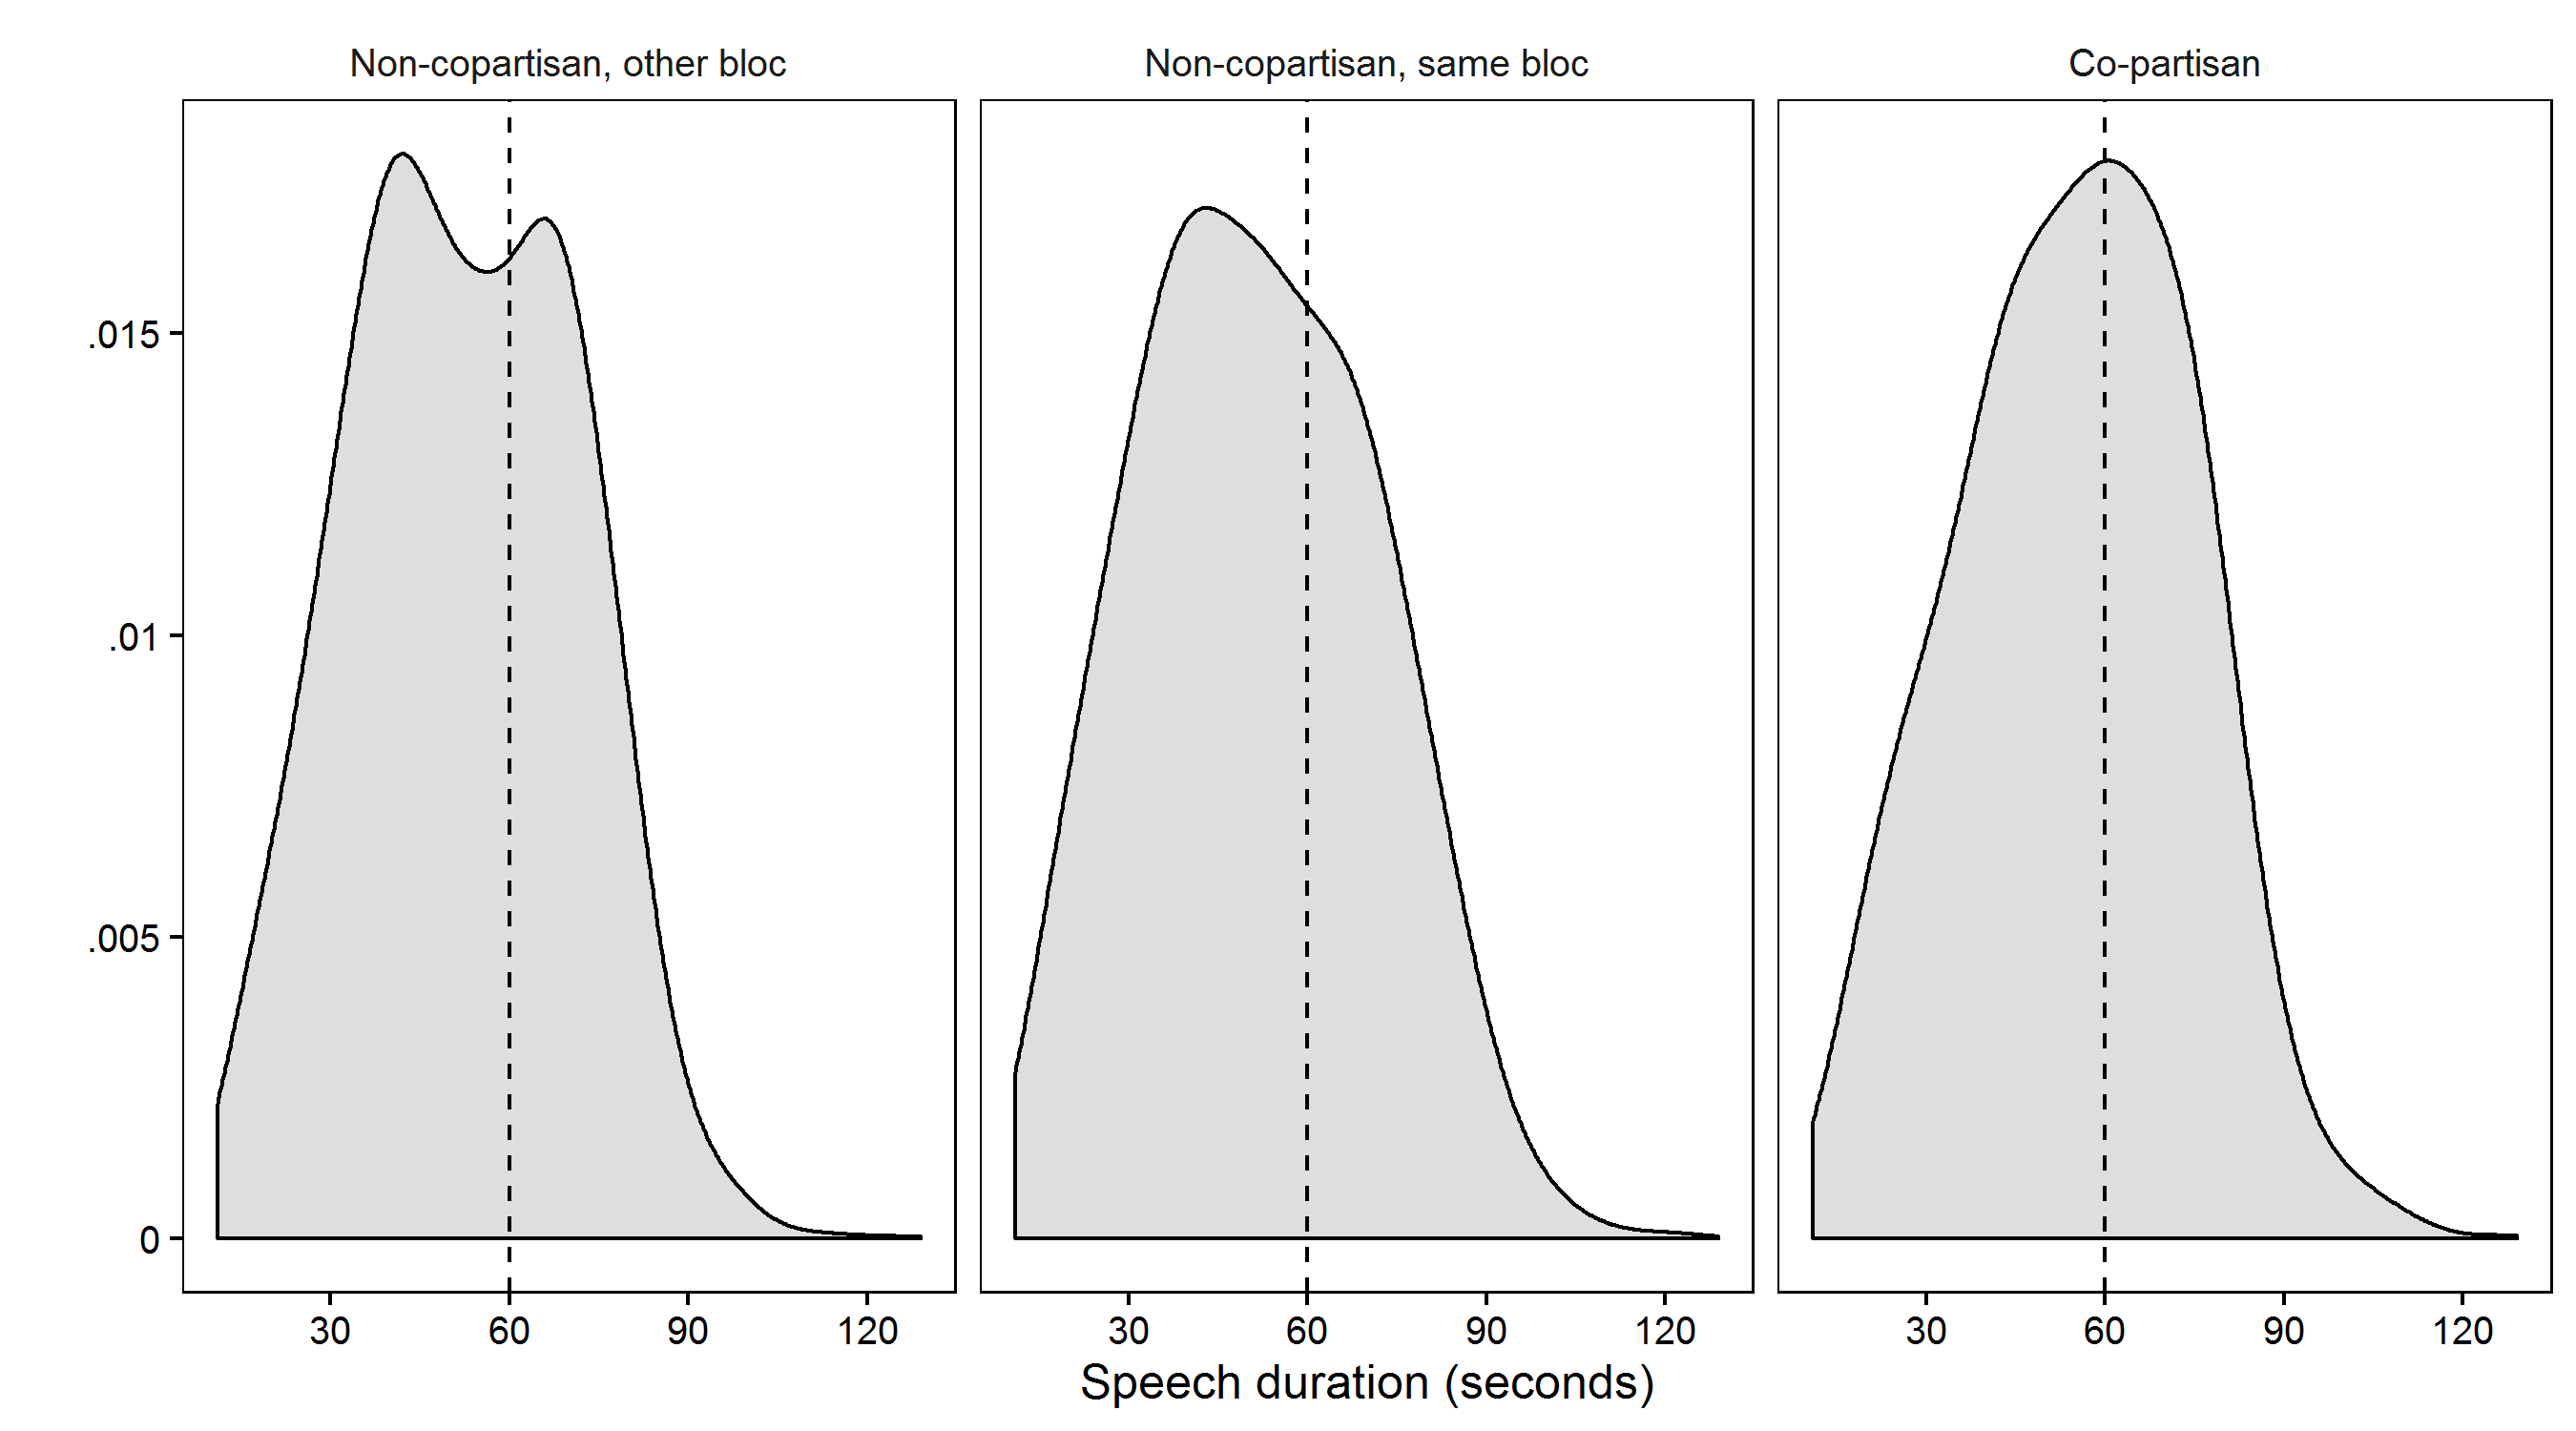
\includegraphics[scale=.70]{../figures/parlbias_dens}
  \caption{Distribution of speaking times for non-copartisans outside of the chairman's political bloc (left panel), non-copartisans from the chairman's own political bloc (middle panel) and copartisans (right panel). The dashed vertical line indicates the 60-second limit for short speeches. Non-copartisans drop off before reaching the limit. No such pattern is apparent for copartisans.}\label{parlbias_dens}
\end{figure}

As seen in Figure \ref{parlbias_dens}, the frequency of non-copartisan speeches drops markedly as speech lengths approach the 60-second limit. By contrast, copartisan speeches are almost perfectly symmetrically distributed around the limit. The figure lends \textit{prima facie} support to the notion that speech lengths depend on the partisan relation between chair and speaker.

A noticeable detail in Figure \ref{parlbias_dens} is that for non-copartisans not in the chairman's political bloc (i.e., left panel), the distribution of speaking times is slightly bimodal. The reason for this slight bimodality is not clear. It is indicative of some heterogeneity in the observed effect, such that the remarks of some non-copartisans are censored to well below the cutoff, whereas others are unaffected. We do not delve further into what underpins this heterogeneity in this paper.

Table \ref{parlbias_regtab1} presents estimations of various specifications of equation \ref{model}. Model 1 presents a bivariate regression of speech length on copartisanship; models 2-5 add various controls. Across all model specifications, the estimated effect of copartisanship is robustly significant and in the predicted direction. 

\input{../tables/parlbias_regtab1.txt}

The results thus support the hypothesis that copartisanship is associated with longer speeches. The estimated effect of copartisanship ranges from 3.3 additional seconds (without any controls) to 2 seconds (with speaker party fixed effects), with a median of 3.1 seconds. In absolute terms, the estimated effects thus seem fairly small, but the effect is equivalent to an appreciable `copartisanship premium' of around 5 percent of the expected speech length.

The models presented in table \ref{parlbias_regtab1} also control for two other possible confounders. For one, one may suspect that the observed copartisanship effect reflects the fact that members of major parties, which hold the chairman positions, speak earlier in the day, and have more energy to use the full extent of their speaking time. Models 2-5, which include a speech order control, suggest that there is in fact a slight `fatigue effect': speeches later in the day are very slightly, though insignificantly, shorter. The latest speeches in the data are on average around two seconds shorter than the earliest. But controlling for order does not affect the significance of the estimated effect of copartisanship.

Second, one could suspect that the effect is driven by minor parties, which do not hold chairman positions, being awarded less speaking time as a matter of sheer proportionality. Such a difference could produce a spurious copartisanship effect. Model 5 accounts for this by estimating the model for only parties which hold chairman positions. As shown, the effect is undiminished.

\subsection{Robustness check: binary speaking time measure}

If the difference in speaking times observed for copartisans vs. non-copartisans reflects biased enforcement of speaking time rules, we should expect the difference to be concentrated around the 60-second threshold. In contrast, if the observed difference instead reflected fewer copartisan speeches lasting five seconds and more lasting 10 seconds, it would not make sense to attribute the difference to biased rule enforcement. Chairmen can only meaningfully affect speaking times in the neighborhood of the 60-second threshold. 

The distributions plotted in Figure \ref{parlbias_dens} strongly suggest that the difference is indeed concentrated around the 60-second threshold. As a way of formally testing the idea, we dichotomize the dependent variable to indicate whether the speaker has exceeded the 60-second limit or not. Table \ref{parlbias_regtab1logit} presents the results from a series of logistic regression models, specifications identical with those in Table \ref{parlbias_regtab1}, estimated with this new dependent variable.

\input{../tables/parlbias_regtab1logit.txt}

As the table shows, the results using the dichotomized dependent variable are substantively similar. The copartisanship coefficient remains significant across all specifications. 
%Since the reported coefficients are logit coefficients they are not readily interpretable. 

\subsection{Making sense of the magnitude of bias}
As a way of providing more intuitive quantities of interest, figure \ref{parlbias_effectplot} plots average marginal effects for all the copartisanship estimates in tables \ref{parlbias_regtab1} and \ref{parlbias_regtab1logit}. As shown in the logit model estimates in the left hand panel, a speaker of the same party as the chairman has an on average five percent higher chance of exceeding the speaking time limit, an estimate that is fairly stable across specification. In the linear model estimates in the right hand panel, the median effect estimate reflects an around 3 seconds longer speaking time for copartisans.

\begin{figure}[!htbp]
\centering
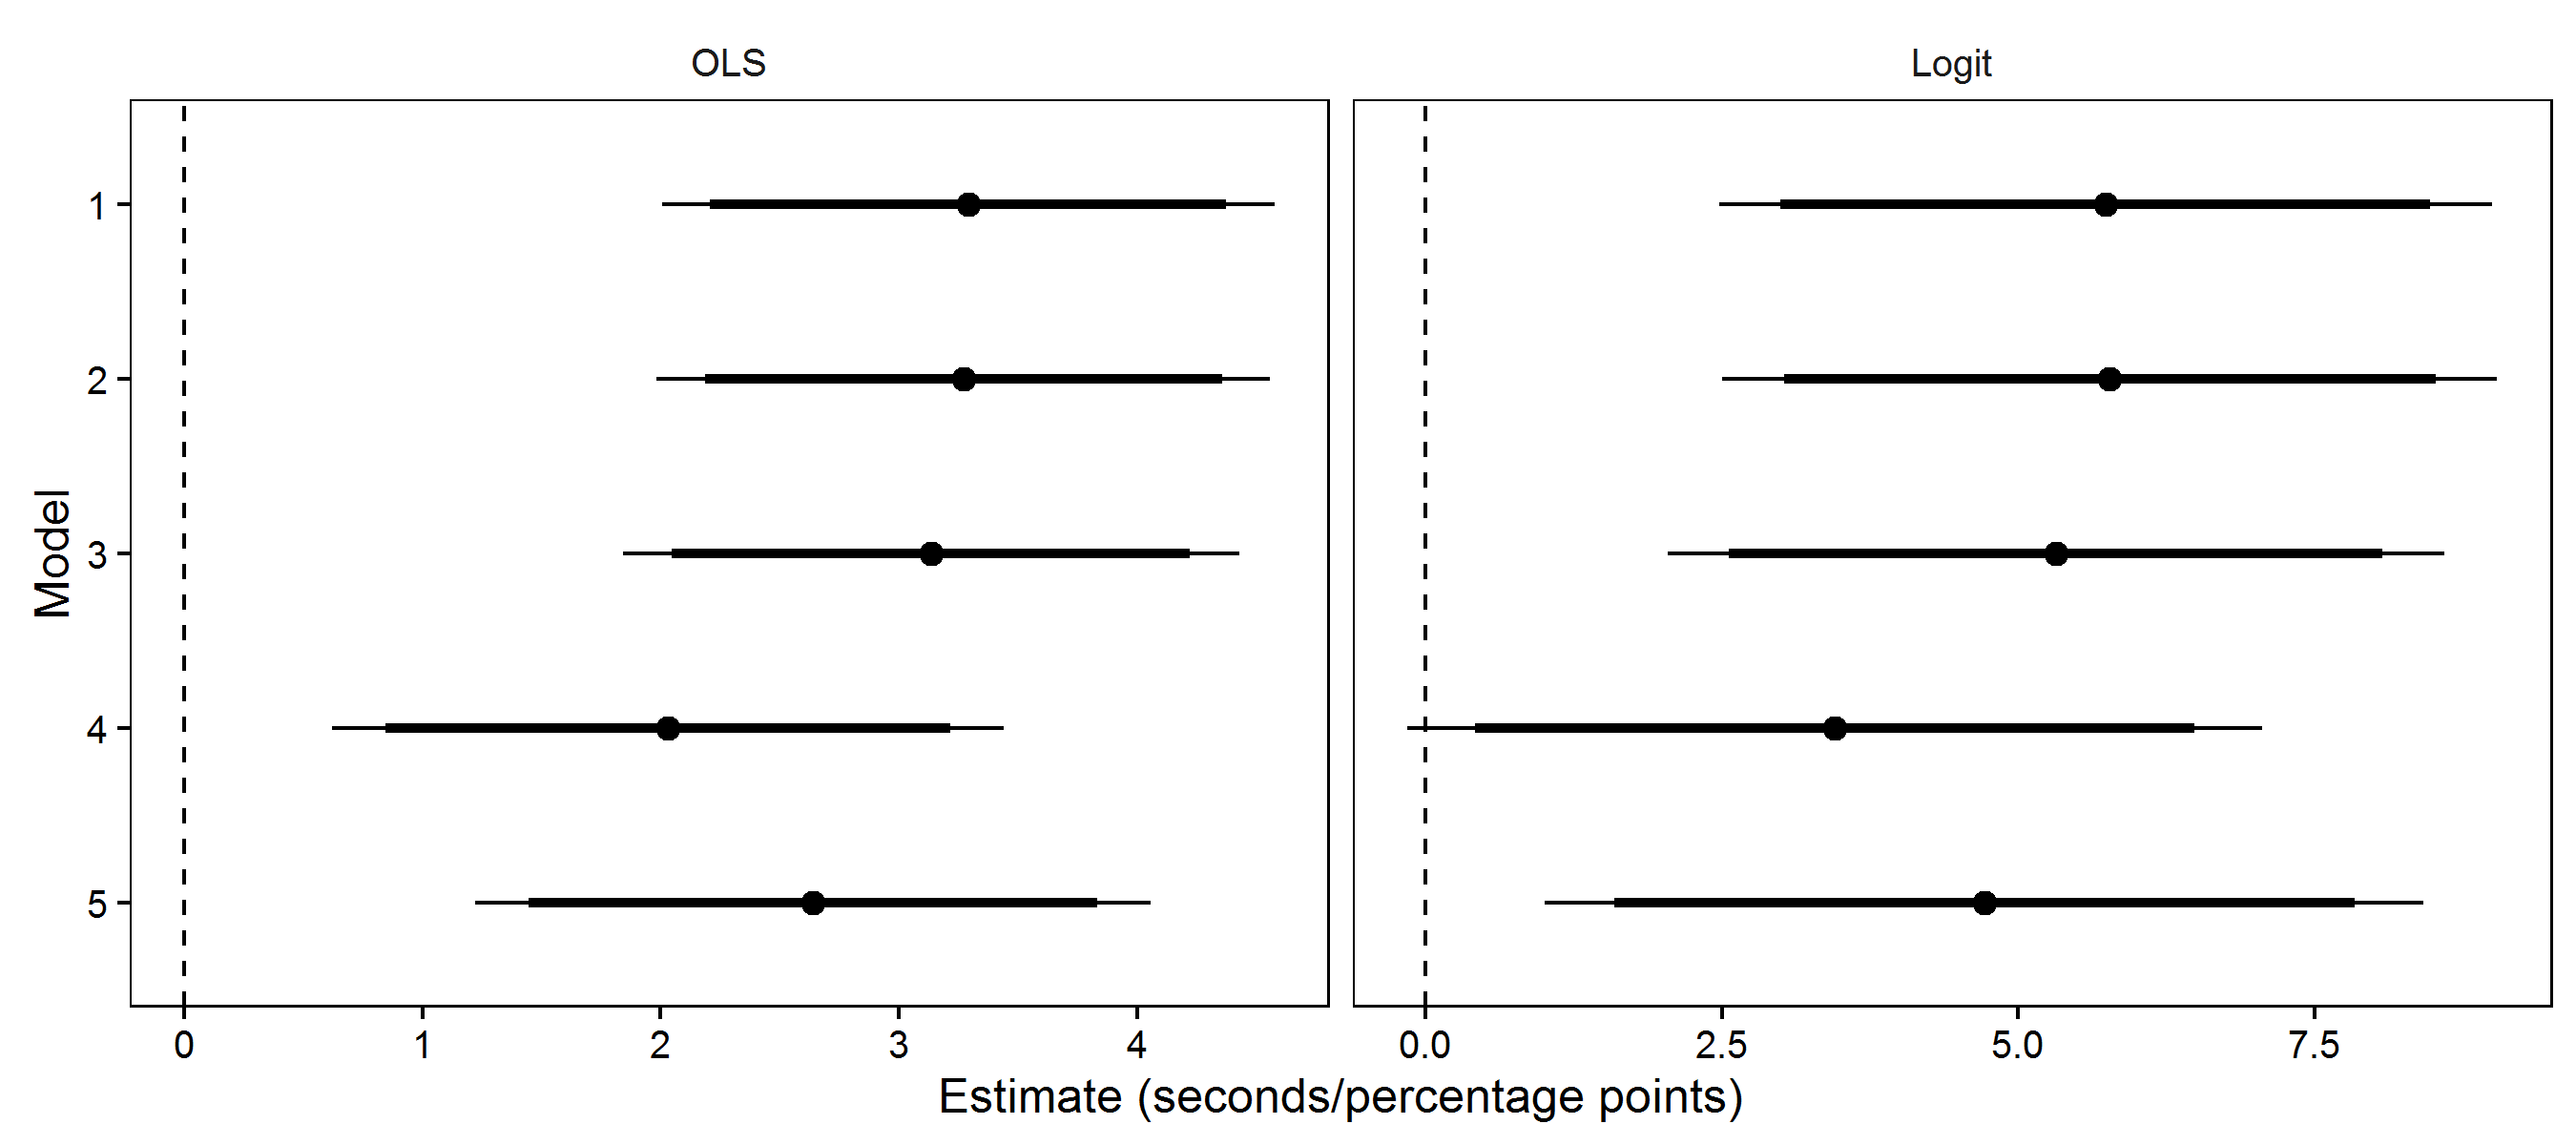
\includegraphics[scale=.65]{../figures/parlbias_effectplot}
  \caption{Estimated effect of copartisanship on speaking time (left panel) and probability of exceeding 60 seconds (right panel) for each of the five models estimated. Error bars represent 90 percent (thick lines) and 95 percent (thin lines) confidence intervals. Logit model estimates represent marginal effects expressed in percentage points.}\label{parlbias_effectplot}
\end{figure}

There are several ways to make sense of the magnitude of this effect. One is in terms of standardized measures of effect size such as Cohen's $d$, which assesses effects relative to the standard deviation of the dependent variable. Since the standard deviation of speaking time is 28.6, Cohen's $d$ for the estimated effect is around 0.1, typically classified as a `small' effect \citep{Cohen1992}. This corresponds well to the intuitive sense that 3 seconds out of a speech of around 60 seconds is indeed a relatively small fraction. At the same time, this characterization somewhat understates the magnitude of the effect, since it ignores the repeated nature of the speeches. Given that each chairman oversees 128 speeches per debate on average, the cumulative speaking time bias per chairman per debate comes to around six minutes. In other words, though the speaking time bias is small at the level of the individual speech, it adds up when viewed from the perspective of each chairman. At the same time, the continual rotation of chairmen means that in the aggregate, the these biases are likely to roughly cancel out. Overall, the magnitude of bias would seem to be best characterized as small, but non-negligible.

\subsection{Political moderators: Distance or party group affiliation? }\label{polmod}

Having established the presence of biased rule enforcement, we return to the question outlined in the introduction: what is the most plausible psychological mechanism? As a way of getting at this question, we test if chairmen appear responsive to variation in the political affiliation of speakers which should be relevant to a politically strategic actor. If the partisan governance account is correct, chairmen would plausibly be most strongly biased against politically distant speakers. Conversely, if the social identity account is correct, chairmen would presumably treat non-copartisans roughly equally, seeing as they are all out-group members, irrespective of political distance. The extent to which the observed effect is moderated by political factors is thus at least suggestive of the mechanism underpinning the observed bias.

The standard way to test if political distance moderates the observed relationship would be to set up an interaction between copartisanship and political distance between chairman and speaker. However, this is statistically infeasible, since copartisanship and political distance are highly conditionally dependent: for all copartisans, political distance is by definition zero, and for all positive values of political distance, copartisanship is by definition zero. Hence, a regression model with copartisanship interacted with political distance is inestimable.

We therefore take a different approach, testing the moderating effect of political distance by reestimating the full model (model 4 in table \ref{parlbias_regtab1}) for various subsets of the data where the political distance between chairman and speaker is artificially restricted.  First, we calculate an approximate distance measure based on averaged voter estimates of party positions from the most recent national election survey \citep{Stubager2013}.\footnote{Respondents in the 2011 Danish National Election Study were asked to place parties on a 0 to 10 scale. From left to right, the party position estimates are: Unity List (1.49), Socialist People's Party (2.79), Social Democrats (3.84), Social Liberals (5.01), Liberal Alliance (7.14), Conservative People's Party (7.23), Liberals (7.35), Danish People's Party (7.74)} For each speaker, we calculate the distance measure as the absolute value of the distance between the parties of speaker and chairman. We then reestimate the full model using only data from chairman-speaker pairs where the distance is less than or equal to the median of all observed distances. Second, to test the robustness of the distance measure, we apply a similar restriction using a rank-transformed (ordinal) version of the distance measure. Finally, we also estimate a model restricting the data to cases where the chairman-speaker pair belong to the same political bloc. Table \ref{parlbias_regtabmods} shows the results of each of these restrictions alongside the full model. We plot the estimates in figure \ref{parlbias_modeffectplot}.

\input{../tables/parlbias_regtabmods.txt}

\begin{figure}[!htbp]
\centering
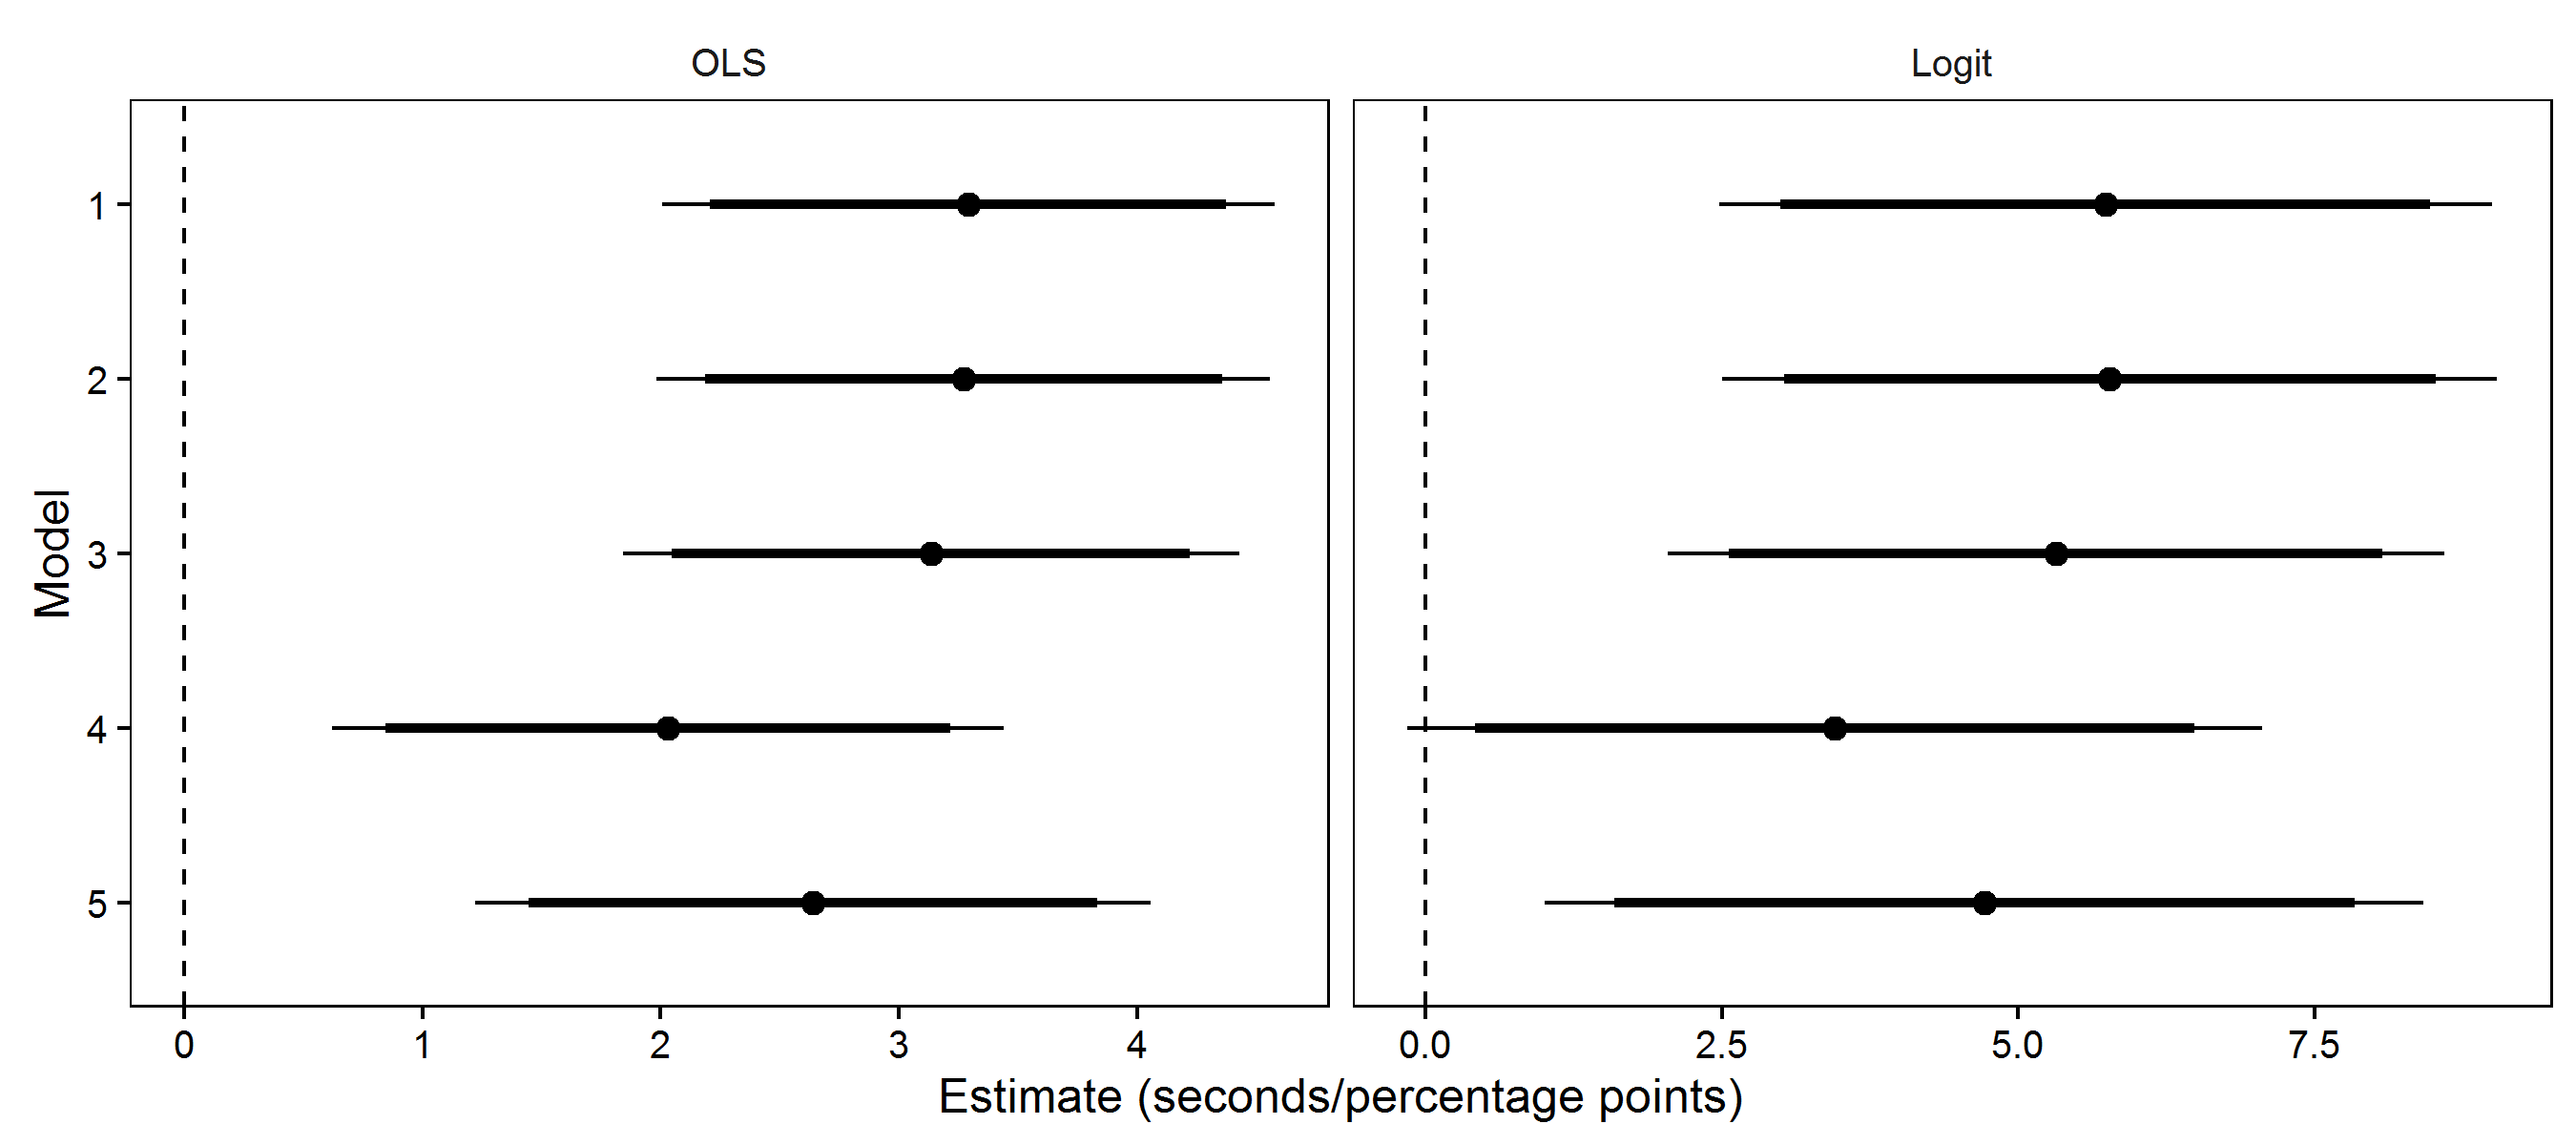
\includegraphics[scale=.65]{../figures/parlbias_modeffectplot}
  \caption{Estimated effect of copartisanship on speaking time under various restrictions on political distance between chairman and speaker. Error bars represent 90 percent (thick lines) and 95 percent (thin lines) confidence intervals.}\label{parlbias_modeffectplot}
\end{figure}


As shown, all of the estimated effects of copartisanship on speaking time are clearly smaller than in the full model, and none of them are statistically significant. The difference should not be overstated: all of the estimates still have the predicted sign, and there is considerable overlap between the confidence intervals. Still, the results do strongly suggest that the effect of copartisanship is weaker when copartisans are compared to politically proximate non-copartisans. As argued above, this pattern is more consistent with the partisan governance account, according to which chairmen should be attuned to how politically distal the speaker is.

Empirically speaking, the conclusion from these moderation tests is reasonably clear: though chairmen exhibit bias against non-copartisans on average, this bias is much less pronounced when comparing copartisans only with non-copartisans who are politically proximate and/or belong to the same political bloc. Strictly speaking, the bias thus appears to be not one of partisanship per se, but of political proximity and/or bloc affiliation.

However, this empirical result is not necessarily highly informative of the merits of the competing theoretical perspectives. The fact that chairmen are sensitive to the political distance and bloc affiliation of the speaker would seem to speak in favor of the partisan governance perspective, since making this distinction furthers a broader political agenda. On the other hand, a social identity perspective might argue that, in parliamentary politics in multiparty systems, political blocs and groups of ideologically similar parties are themselves meaningful social identities. Thus, though the results do lend some support to the partisan governance account, it seems safest to conclude that the tests cannot fully adjudicate between the two theorized mechanisms.

\subsection{Additional tests}

\todo{explain figs and tabs in appendix}

Section \ref{appact}

Section \ref{approbust}

Section \ref{appchairranef}



robustness checks

Figure \ref{parlbias_chairranfefs} in the appendix shows effects estimated separately for each chairman in the data.


\section{Conclusion}\label{conc}

\noindent The key finding from this study is that speaking time rules in Danish parliamentary debates are not enforced equally. Specifically, speeches are around 2.8 seconds longer on average when the person speaking shares party affiliation with the chairman enforcing the rules. This corresponds to a roughly five percent greater chance for copartisans of exceeding the 60-second speaking time limit.

Since the official rules call for neutral enforcement of the limit, this difference can be attributed to intergroup bias on the part of the rule enforcer, i.e. the chairman. The intergroup bias explanation is consistent with a wealth of laboratory experimental evidence demonstrating the impact of group identity on distributional preferences. We contribute to this literature by showing intergroup bias among elected political officials in a natural setting. The generalizability of the finding is further bolstered by the fact that the empirical setting is characterized by clear rules of universality, complete observability, low societal-level corruption, and a strong tradition of parliamentary cooperation -- thus in several respects a `least likely' case for intergroup bias in rule enforcement.

\todo{implications re: canceling out}

Two concerns about the nature of the observed effect linger. First of all, the data is uninformative as to whether the observed difference reflects actual biased enforcement on behalf of chairmen as opposed to speakers voluntarily cutting their speeches short in anticipation of biased enforcement. In the latter, copartisans could theoretically gain an advantage solely by virtue of anticipating more lenient rule enforcement, even if rules are in fact enforced equally. \todo{4.1 more self selec}

Second, and more theoretically crucial, assuming chairs to treat copartisans and non-copartisans unequally, the study cannot identify whether the unequal treatment is intentional. While both intentional and unintentional mechanisms could meaningfully be conceived as intergroup bias, they point to very different substantive interpretations of the evidence. In the partisan governance perspective, chairmen deliberately skew the rule enforcement in favor of their own party in order to gain a political advantage. In the social identity perspective, chairpersons are subconsciously swayed by group identities, even while honestly trying to enforce the rules equally.

%soften this - mechanism is a task for future studies
To be sure, the distinction between these two mechanisms is not necessarily a perfectly exclusive one: biased behavior may reflect a murky combination of strategic and implicit motives. Still, the theoretical distinction is too important to gloss over. A promising avenue for future research is thus to find ways to distinguish more clearly which of the two mechanisms dominate. In a broader sense, future research would do well to examine other ways in which psychological phenomena, replicated in laboratory studies many times over, manifest themselves in political behavior observable in natural settings.

%Regardless of the specific composition of these mechanisms, the conclusion remains that even when institutional norms militate strongly against bias, governance entirely blind to group loyalties remains an elusive ideal.

%PAPER ALSO SHOWS HOW LEGISLATURES CAN BE STUDIED AS LABORATORIES OF SOCIAL BEHAVIOR UNDER INTITUTIONAL CONSTRAINT

\newpage
\begingroup
\parindent 0pt
\parskip 2ex
\def\enotesize{\normalsize}
%\theendnotes %from endnotes package
\endgroup

\clearpage

%\singlespacing

\bibliographystyle{../../thesis/bibliography/model2-names}
\bibliographystyle{chicago}
\bibliography{../../thesis/bibliography/library}

\clearpage

\appendix

\section{Appendix}

\subsection{Predicting chairman activity}\label{appact}

Here I present results from regression models predicting how many debates chairpersons control. The key result from these models is that the main predictor of number of debates controlled is how long a chairperson has been a member of the leadership. There is an additional small premium for being the head chairperson, which likely reflects the fact that by convention, the president always takes the first shift controlling a debate. In contrast, number of seats has no significant association.

\input{../tables/parlbias_remarksregtab.txt}

Table 1 shows that the main determinant of the number of remarks enforced by a chairmen is chairman's tenure, i.e. for how many debates he or she was in the leadership. In contrast, party seat share is uncorrelated with activity. The results complement the qualitative evidence from correspondence with the parliament leadership that chairperson activity is largely driven by 'supply-side' factors, i.e. chairpersons' availability on the day of the debate, and not by party specific factors such as their parliamentary power.

\clearpage

\subsection{Robustness checks of main results}\label{approbust}

Here we present additional robustness checks of the main results. Table \ref{parlbias_regtabrs} presents results restricting the sample to remarks given by members of parties in the parliamentary leadership (i.e., the five biggest parties by number of seats).

\input{../tables/parlbias_regtabrs.txt}

Table \ref{parlbias_regtabdfe} \todo{finish}

\input{../tables/parlbias_regtabdfe.txt}

Table \ref{parlbias_regtabexpm} \todo{finish}

\input{../tables/parlbias_regtabexpm.txt}

\clearpage
\subsection{Effect heterogeneity across parties and chairmen}\label{appchairranef}

Here we assess the heterogeneity of the observed effect across parties and individual chairmen. Figure \ref{partyranefs} and Figure \ref{parlbias_chairranfefs} \todo{wrap}.

\begin{figure}[!h]
\centering
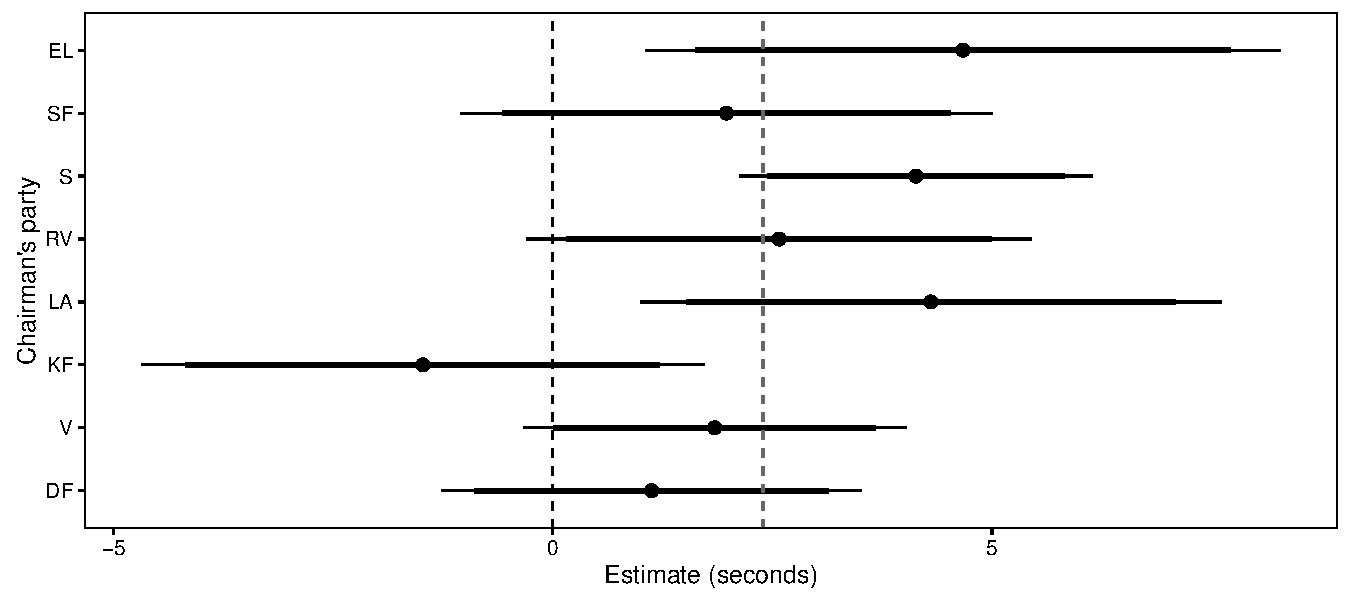
\includegraphics[scale=.55]{../figures/parlbias_partyranefs.pdf}
\caption{Effects of copartisanship estimated separately for each chairman's party. Estimates are drawn from a random effects model corresponding to model 3 in Table 2 with varying slopes for chairman party. The grey dashed vertical line shows the average copartisanship effect (i.e., the fixed effect). Parties are ordered top to bottom according to party ordinal left/right ranking. Error bars represent 90 percent (thick lines) and 95 percent (thin lines) confidence intervals.}\label{partyranefs}
\end{figure}

\begin{figure}[!h]
\centering
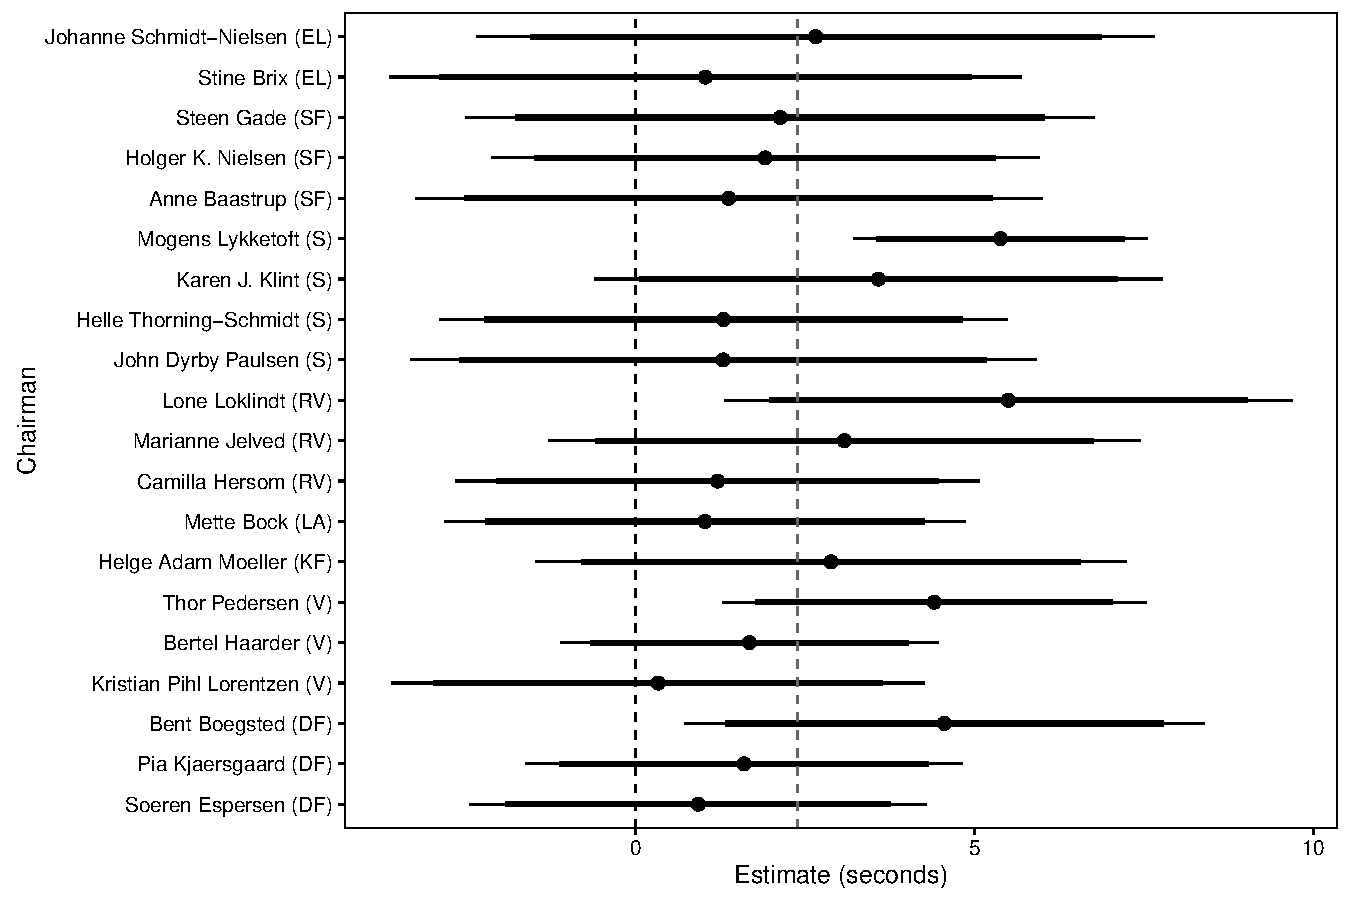
\includegraphics[scale=.55]{../figures/parlbias_chairranefs}
  \caption{Effects of copartisanship estimated separately for each chairman in the data. Estimates are drawn from a random effects model corresponding to model 3 in Table 2 with varying slopes for individual chairmen. The grey dashed vertical line shows the average copartisanship effect (i.e., the fixed effect). Chairmen are ordered top to bottom according to party ordinal left/right ranking and within parties according to estimated effect. Error bars represent 90 percent (thick lines) and 95 percent (thin lines) confidence intervals.}\label{parlbias_chairranfefs}
\end{figure}


\end{document}